\documentclass[titlepage]{article}
\usepackage[utf8]{inputenc}
\usepackage{graphicx}
\usepackage{ skull }
\usepackage[spanish]{babel}
\usepackage{lipsum}
\usepackage{amsmath}
\usepackage{amssymb}

\usepackage{natbib}

\title{blanco2 taller}
\author{Patricio Whittingslow}
\date{October 2019}

\begin{document}

\begin{titlepage}
\centering
{Instituto tecnológico de Buenos Aires \par}
\vspace{5cm}

 {\Huge \bf Mi Titulo \par }
 
\vspace{2cm}

{\Large \sc Autor: Pato \par}

\vspace{1cm}

\end{titlepage}

\begin{abstract}
    \lipsum[1]
\end{abstract}

\tableofcontents

\clearpage

\section{Introduction}
\subsection{sec 2}
\begin{figure}[h!] 
    \centering
    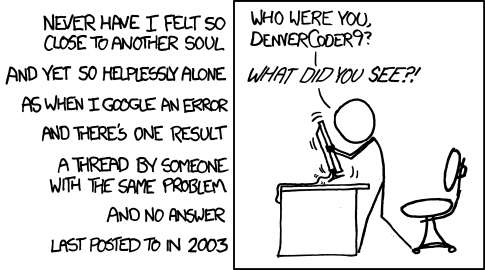
\includegraphics[width=\textwidth]{comic.png}
    \caption{Mi epigrafe.}
    \label{fig:miComicFavorito}
\end{figure}

Como pueden ver, en la figura \ref{fig:miComicFavorito}

\vspace{5mm}

\begin{tabular}{lll}
	\multicolumn{3}{l}{Todo Latex} \\ \hline
	32       & 64       & 128      \\
	2        & 4        & 8       
\end{tabular}
\begin{verbatim}
	\begin{tabular}{lll}
	\multicolumn{3}{l}{Todo Latex} \\ \hline
	32       & 64       & 128      \\
	2        & 4        & 8       
	\end{tabular}
\end{verbatim}

\vspace{5mm}
Hola Hola 


\begin{table}[h!]
\centering
\caption{Otro grande epigrafe}

\begin{tabular}{|l|l|l|l|l|}
\hline
\multicolumn{3}{|l|}{Asistentes Externos al Taller de LaTeX} & 222 & 2232 \\ \hline
Nombre                        & DNI        & Presente        &     &      \\ \hline
Luz Carvajal                  &            &                 &     &      \\ \hline
Paula Oseroff                 &            &                 &     &      \\ \hline
María Agustina Valdés         &            &                 &     &      \\ \hline
\end{tabular}
\label{tab:asistentes}
\end{table}
\section{Sec2}
\subsection{sec 2}
Se hace referencia a la tabla \ref{tab:asistentes} y a la figura \ref{fig:miComicFavorito}


La ecuación de la energía es \( E=mc^2 \). Tomada del libro Raymond S. Serway. Hay ecuaciones más grandes como: 
\[ \int_{\gamma}^{99} x_0 = 9  \]
\[ \alpha, \Gamma ,\Phi \phi \varphi \skull \]
Otra forma de crear una ecuación
\begin{equation}
    \Phi = \oint \omega dx
\end{equation}

\begin{equation*} \label{eq:miGranEcuacion}
    \Phi = \oint \left( \frac{22 \cdot \Gamma}{\hbar} \right) dx
\end{equation*}

Referenciando (\ref{eq:miGranEcuacion}).

\textbf{Agregando el paquete natbib al preambulo y un archivo bibtex}: Si no cito el libro \cite{masas}, no va aparecer en mi lista de referencias. Tambíen puedo citar con \citep{masas}.%


\bibliography{biblio.bib} % Indica archivo
\bibliographystyle{plainnat}  %estilo de bibliografia

\begin{verbatim}
 \cite{masas}  vs  \citep{masas}.

	\bibliography{biblio.bib} % Indica archivo
	\bibliographystyle{plainnat}  %estilo de bibliografia
\end{verbatim}

\end{document}
